\chapter{Grundlagen}
\label{grundlagen_cha}

Im folgenden Kapitel werden die Grundlagen beschrieben, die uns zur Verfügung standen, um die im ersten Kapitel näher beschriebene Zielsetzung zu erreichen.
Dies betrifft zum einen die Software-Grundlage MCA2, die vorhandenen Software-Projekte \lstinline{Odete} und \lstinline{SegwayOmni}, sowie die mobile Roboterplattform \gls{hollie}.
 
\section{\glstext{hollie}}
\label{grundlagen_hollie_sec}
\authorsection{\editorjulian, \editortobias}
\begin{quotation}
\itshape
\gls{hollie} ist ein mobiler, zwei-armiger Service-Roboter, der als Teil des \gls{fzi} House of Living Labs (\gls{holl}) in Karlsruhe entwickelt wurde und die Robotik, \gls{aal}-- und Mobilitätsdienste am \gls{fzi} verbindet. In Zukunft wird dieser Roboter im \gls{holl} verschiedene Begleit--, Assistenz-- und Serviceaufgaben übernehmen, daher auch der Name \gls{hollie} --- \glqq House of Living Labs intelligent Escort\grqq .

Dank der zwei 6-Achsen-Industrie-Roboterarme, einer zuverlässigen omnidirektionalen Basisplattform mit Mecanum-Rädern und den mehrfingrigen Händen besitzt \gls{hollie} eine beeindruckende Beweglichkeit und ist extrem anpassungsfähig und flexibel. Durch den Einsatz erprobter und robuster Industrie-Komponenten kann \gls{hollie} schnell und zuverlässig die zugewiesenen Aufgaben meistern.

Zwei Laserscanner bilden die Datengrundlage für die sichere Navigation im gesamten \gls{fzi} House of Living Labs (\gls{holl}). So kann \gls{hollie} in Zukunft Besuchergruppen durch das \gls{holl} führen und die verschiedenen Laborbereiche selbständig mit Hilfe der internen Sprachausgabe präsentieren.
\normalfont(\cite{fziHoll2})
\end{quotation}

\begin{figure}[h]
	\center
	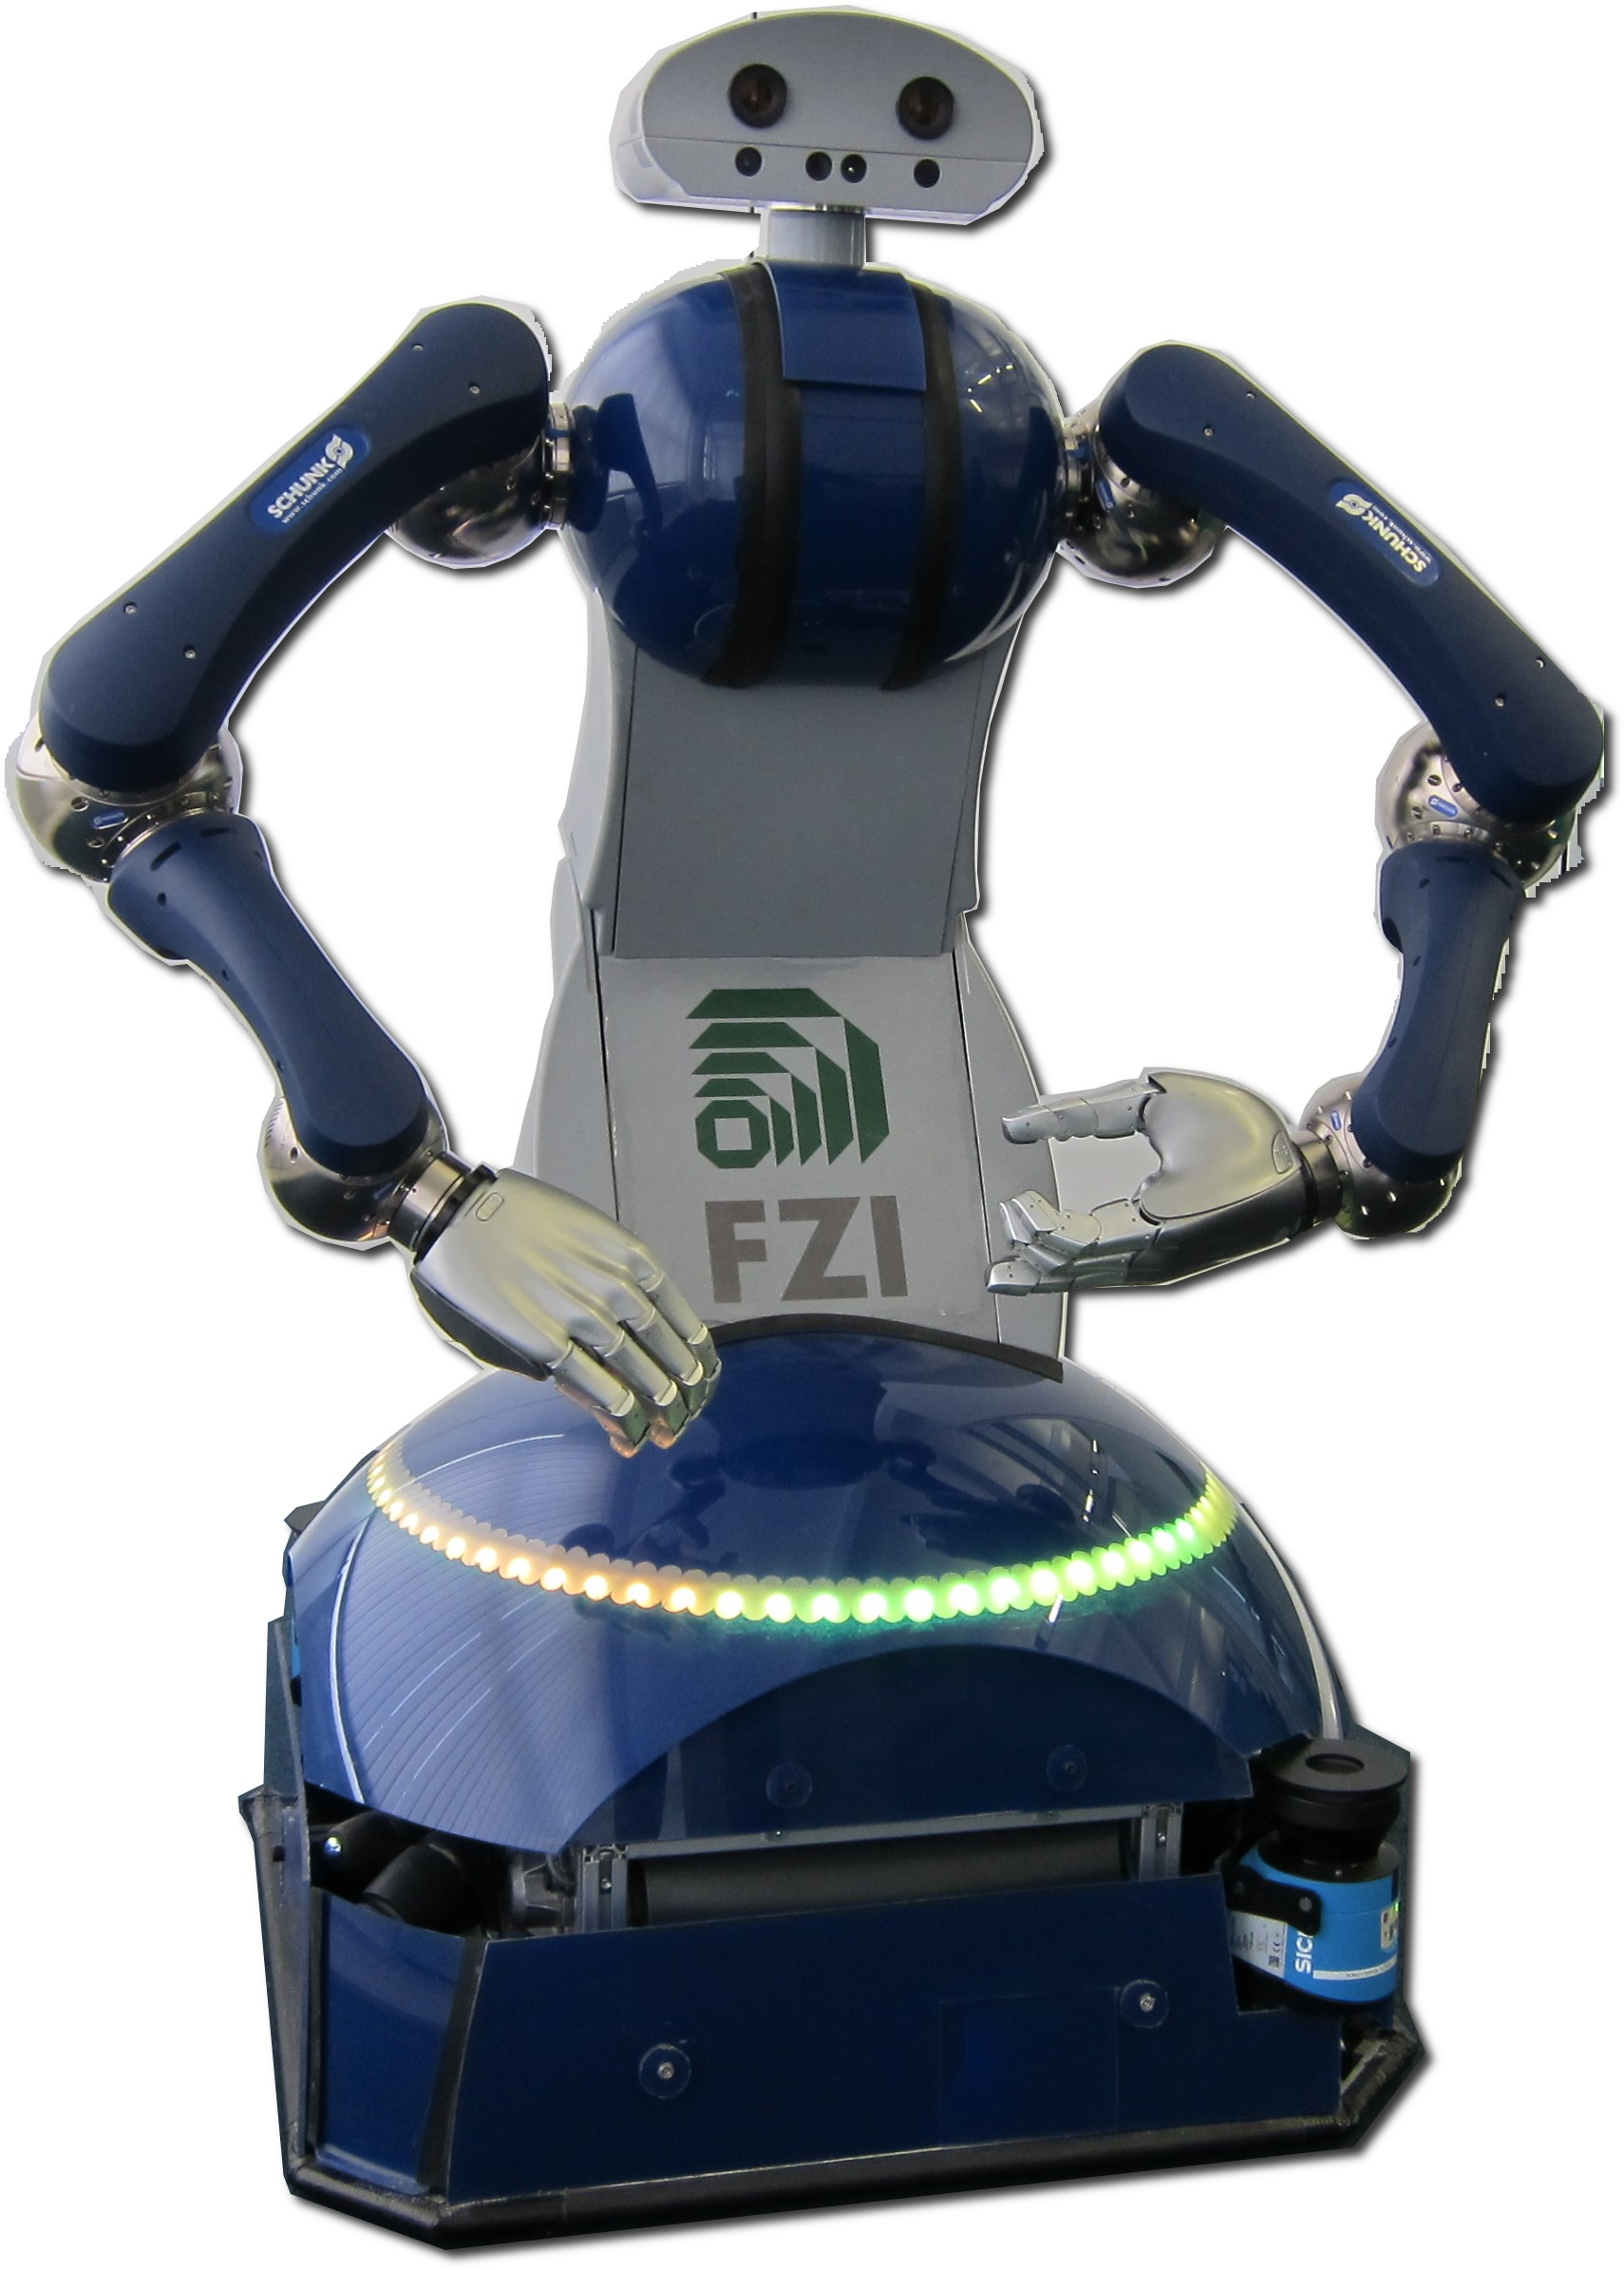
\includegraphics[width=0.5\textwidth]{graphics/hollie}
	\caption{\label{fig:hollie} Die mobile Roboterplattform \gls{hollie}}
\end{figure}

\section{MCA2 - Modular Controller Architecture Version 2}
\authorsection{\editoranne}

Entwickelt, um die Bedürfnisse nach Wiederverwendbarkeit und Erweiterbarkeit eines Softwareprojekts zu unterstützen,
 ist MCA2 ein modulares Software-Rahmenwerk. Dieses unterstützt wiederverwendbare Komponenten mit standardisierten Komponenten,
 die leicht erweiterbar sind. Dadurch wird das Programmieren auf unterschiedlichen Roboter-Prototypen effektiver.

Erreicht wird dies, indem Teile des gesamten Kontrollsystems in kleinen standardisierte Modulen organisiert wird.
 Diese Module können dann im entsprechenden Kontext immer wieder verwendet werden, ohne erneut angepasst werden zu müssen.
 Das Rahmenwerk MCA2 sorgt für die Kommunikation und Synchronisation zwischen diesen Teilen.

\begin{figure}[h]
	\center
	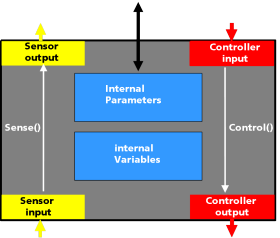
\includegraphics[scale=2.0]{graphics/mcamodule.png}
	\caption{\label{fig:MCA-Modul} Beispiel für ein MCA Modul}
\end{figure}

Jedes Modul ist dabei in gleicher Weise aufgebaut. Es besitzt 5 Schnittstellen, wovon vier zur Kommunikation mit anderen Modulen dienen,
 die fünfte wird genutzt um interne Parameter zu lesen und zu ändern. Die vier Kommunikationsschnittstellen ergeben sich jeweils aus der
 Kommunikation zu über- oder untergeordneten Modulen. In jede dieser beiden Richtung können Daten gesendet, bzw. empfangen werden.
 Man spricht in der einen Richtung von Sensor-, in der anderen Richtung von Kontroll-Daten. Diese Daten sind dabei realisiert durch einen Vektor fester Werte,
 die von einem Modul an ein Weiteres in derselben oder einer permutierten Reihenfolge weitergegeben werden.
 Mittels der fünften Schnittstelle werden diese Daten dann manipuliert. Dazu besitzt jedes Modul zwei Funktionen: Die Sense()- und die Control()-Funktion.
 Die Sense()-Funktion dient dazu, die Sensordaten von der Input- zur Output-Schnittstelle verändert oder unverändert weiter zu geben, die Control()-Funktion ist
 analog für die Kontrolldaten zuständig.

Das große Ziel von MCA2 war die Wiederverwendbarkeit von Modulen, dies wird um so effektiver, je einfacher die einzelnen Module gehalten sind.
 Um dennoch ein leistungsfähigeres Modul zu erhalten, das eine komplexere Funktionalität beinhaltet, werden Module in Gruppen zusammengestellt. 

\begin{figure}[h]
	\center
	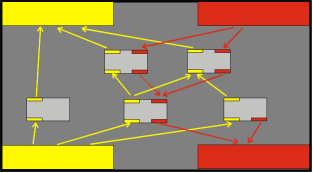
\includegraphics[scale=2.0]{graphics/mcagroup.png}
	\caption{\label{fig:MCA-Gruppe} Beispiel für eine MCA Gruppe}
\end{figure}

Eine Gruppe ist dabei wiederum aufgebaut wie ein Modul, besteht selbst jedoch aus vielen kleinen Modulen,
 um die komplexere Funktionalität zu erfüllen. Wird die Sense()- oder Control()-Funktion einer Gruppe aufgerufen,
 so löst das die Ausführung aller Sense()- und Control()-Funk"-ti"-o"-nen
 innerhalb der Gruppe aus, beginnend bei der Eingangs-Schnitt"-stel"-le, bis hin
 zur Ausgabe-Schnittstelle der Sensor-, bzw. Kontrolldaten.

Die Idee von Gruppen wird in MCA2 dann konsequent weiter gedacht und resultiert darin,
 dass Module und Gruppen wiederum hierarchisch zusammengesetzt werden, um noch komplexere Programme realisieren zu können.
 Eine ausführbare Datei, die aus Gruppen und Modulen zusammengesetzt ist, wird Part genannt.
 Der größte Unterschied zwischen einer Gruppe und einem Part besteht darin, dass die Sense()- und Control()-Funktionen einer Gruppe nur bei Aufruf,
 bei einem Part dagegen immer wiederholt entsprechend einer Art 'Takt' ausgeführt werden.

Für die Arbeit im Rahmen des Projektpraktikums wurde noch ein zusätzlicher Mechanismus benötigt,
 der einen geteilten Speicherbereich anbietet. Organisiert als einfacher Array von festen Werten bieten Blackboards diese Möglichkeit,
 um Daten für komplexere Datenstrukturen wie Bilder weiter zu leiten.
 Benötigt zum Beispiel für das Virtual Protective Field oder auch die Weitergabe von Daten der Laserscanner.

Letztendlich bietet MCA noch Schnittstellen, die via Ethernet alle Sensordaten in Text oder Bild auf einer grafische Benutzeroberfläche bereitstellen.
 Diese mcagui kann auf jedem PC innerhalb des Netzwerkes ausgeführt werden, so dass die ausführende Computereinheit
 mit dem zusätzlichen Overhead nicht belastet wird. Mit Hilfe dieser grafischen Benutzeroberfläche wurde das Testen
 innerhalb einer Simulationsumgebung ausgeführt, aber auch erste Tests auf dem realen Roboter konnten mittels dieser Schnittstelle erleichtert werden.
 Siehe Abbildung \ref{fig:mcagui} \citep{mca}


\section{Odete}
\authorsection{\editordirk}
\todo[inline]{Dirk: Schreiben}


\section{SegwayOmni}
\authorsection{\editordirk}
\todo[inline]{Dirk: Schreiben}

